\chapter{Introduction}\label{chapter:introduction}

This is the first chapter of the \gls{thesis}.~\cite{Aaboud:2016mmw,Bruning:782076}

\section{Creating Figures}\label{sec:figures}
\begin{figure}[htpb]
 \centering
 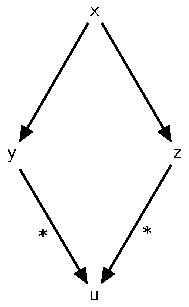
\includegraphics{introduction/example.pdf}
 \caption[Example placeholder figure with a citation~\cite{Higgs:1964ia} and shorter List of Figures caption.
  The List of Figures is protected from first use of glossary entries or acronyms like \acrlong{LHC}.]{%
  This is a placeholder figure to act as an example.
  Here we cite a new reference in the caption to demonstrate that given the package configuration our order of references will not be distributed by the table of contents~\cite{Higgs:1964ia}.}\label{fig:test_figure}
\end{figure}

As can be seen in \Cref{fig:subfigure_example}, the subfigures are independent of each other such that \Cref{fig:subfigure_1} and \Cref{fig:subfigure_2} can be accessed separately.

\begin{figure}[htbp]
 \centering
 \begin{subfigure}[t]{0.48\textwidth}
  \centering
  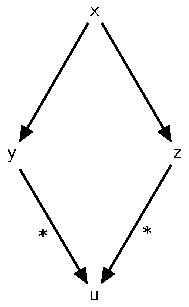
\includegraphics[width=0.3\textwidth]{introduction/example.pdf}
  \caption[Short List of Figures captions work with subfigures too.]{%
   This is the first figure of two, in this example, and its own independent subfigure.}
  \label{fig:subfigure_1}
 \end{subfigure}%
 \quad
 \begin{subfigure}[t]{0.48\textwidth}
  \centering
  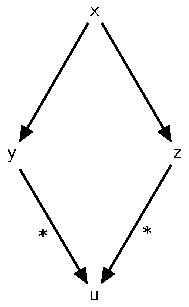
\includegraphics[width=0.3\textwidth]{introduction/example.pdf}
  \caption[Which makes the List of Figures readable and actually helpful.]{%
   As the \texttt{t} alignment option was chosen for the subfigures, they are still properly aligned vertically even though this caption is longer.}
  \label{fig:subfigure_2}
 \end{subfigure}
 \caption{An example of a figure that consists of two subfigures.}
 \label{fig:subfigure_example}
\end{figure}

As an example of an equation formatted in ``\href{https://www.overleaf.com/learn/latex/Display_style_in_math_mode}{display style}'' the equation for the fiducial cross section from~\cite{Aaboud:2016mmw} is reproduced as \Cref{eq:fiducial_cross_section}:
\begin{equation}
 \sigma_{\mathrm{inel}}^{\mathrm{fid}} \left(\zeta > 10^{-6}\right) = \frac{N - N_{\mathrm{BG}}}{\epsilon_{\mathrm{trig}} \times \mathcal{L}} \times \frac{1 - f_{\zeta < 10^{-6}}}{\epsilon_{\mathrm{sel}}}
 \label{eq:fiducial_cross_section}
\end{equation}

\section{Creating Tables}\label{sec:tables}

To create tables in \LaTeX{} it is highly recommended to use the \href{https://www.ctan.org/pkg/booktabs}{\texttt{booktabs}} package.
It allows for very elegant and clean table creation, such as \Cref{table:natural_units}.
If you want to create a table quickly, or have a CSV file that you'd like to quickly turn into a table there are various \href{https://www.tablesgenerator.com/}{online \LaTeX{} table generators}.

\begin{table}[htpb]
 \centering
 \caption[Common quantities in particle physics in natural and SI units.]{%
  Common quantities in particle physics given in both natural units and SI units.}
 \begin{tabular}{@{}llll@{}} \toprule
  Quantity         & Natural Units                 & Natural Units (dimensionful)            & SI Units                                              \\ \midrule
  Speed            & $1$                           & $c$                                     & $3.0\times 10^{8}~\mathrm{m}/\mathrm{s}$              \\
  Angular Momentum & $1$                           & $\hbar$                                 & $10^{34}~\mathrm{m}^2 \,\mathrm{kg}/\mathrm{s}$       \\
  Energy           & $\mathrm{GeV}$                & $\mathrm{GeV}$                          & $1.6\times 10^{-10}~\mathrm{J}$                       \\
  Momentum         & $\mathrm{GeV}$                & $\mathrm{GeV}/c$                        & $1\times 10^{-19}~\mathrm{kg}\,\mathrm{m}/\mathrm{s}$ \\
  Mass             & $\mathrm{GeV}$                & $\mathrm{GeV}/c^{2}$                    & $1.8\times 10^{-27}~\mathrm{kg}$                      \\
  Time             & $1/\mathrm{GeV}$              & $\hbar/\mathrm{GeV}$                    & $6.6\time 10^{-25}~\mathrm{s}$                        \\
  Length           & $1/\mathrm{GeV}$              & $\hbar c/\mathrm{GeV}$                  & $2\times 10^{-16}~\mathrm{m}$                         \\
  Electric Charge  & $1$                           & $e/\sqrt{4\pi \alpha_{\mathrm{em}}}$    & $5.3\times 10^{-19}~\mathrm{C}$                       \\
  Magnetic Field   & $\left(\mathrm{GeV}\right)^2$ & $\left(\mathrm{GeV}\right)^2/\hbar c^2$ & $5\times 10^{16}~\mathrm{T}$                          \\
  \bottomrule
 \end{tabular}\label{table:natural_units}%
\end{table}

Good table design requires some thought and work, so it may be worth a look through some examples:
\begin{itemize}
 \item \href{https://tex.stackexchange.com/questions/238503/tip-on-how-to-make-a-visually-good-table}{TeX StackExchange: Tip on how to make a visually good table}
 \item \href{https://twitter.com/edwardtufte/status/451820483109847040?lang=en}{Edward Tufte endorsed} example from \href{http://static1.squarespace.com/static/56713bf4dc5cb41142f28d1f/t/56fd4c83746fb9261146eed5/1459440776291/ClearOffTheTableMd.gif}{Darkhorse Analytics}
\end{itemize}

\section{Dealing with Widows and Orphans}\label{sec:widos_and_orphans}

To reduce the difficulty of dealing with widowed text (the last line of a paragraph at the start of a page) and orphaned text (the first line of paragraph at the end of a page) the \href{https://ctan.org/pkg/nowidow?lang=en}{\texttt{nowidow}} package is used.
However, that doesn't solve the issue of orphaned section titles.
The user must manually do this, but the following \href{https://texfaq.org/FAQ-widows}{simple advice from \TeX{} FAQ} is recommended:

\begin{quote}
 Once you've exhausted the automatic measures, and have a final draft you want to ``polish'', you should proceed to manual measures.
 To get rid of an orphan is simple: precede the paragraph with \texttt{\textbackslash clearpage} and the paragraph can’t start in the wrong place.
\end{quote}
